\newpage
\section{Auswertung}
\subsection{Emissionsspektrum Kupfer-Röntgenröhre}
Für das Spektrum der Kupfer-Röntgenröhre ergibt sich, das gemessenen
Intensitätsmaximum bei $I_{\text{max}}=218\;$Imp/s, dafür ergibt sich
der zugehörige Braggwinkel $\Theta_{\text{max}}$ und die Wellenlänge $\lambda_{\text{max}}$
\begin{align*}
    \Theta_{\text{max}}=28,2°, && \lambda_{\text{max}}=190,3\si{pm},&&E_{\text{max}}=6,52\si{keV}.
\end{align*}
\begin{figure}[H]
    \centering
    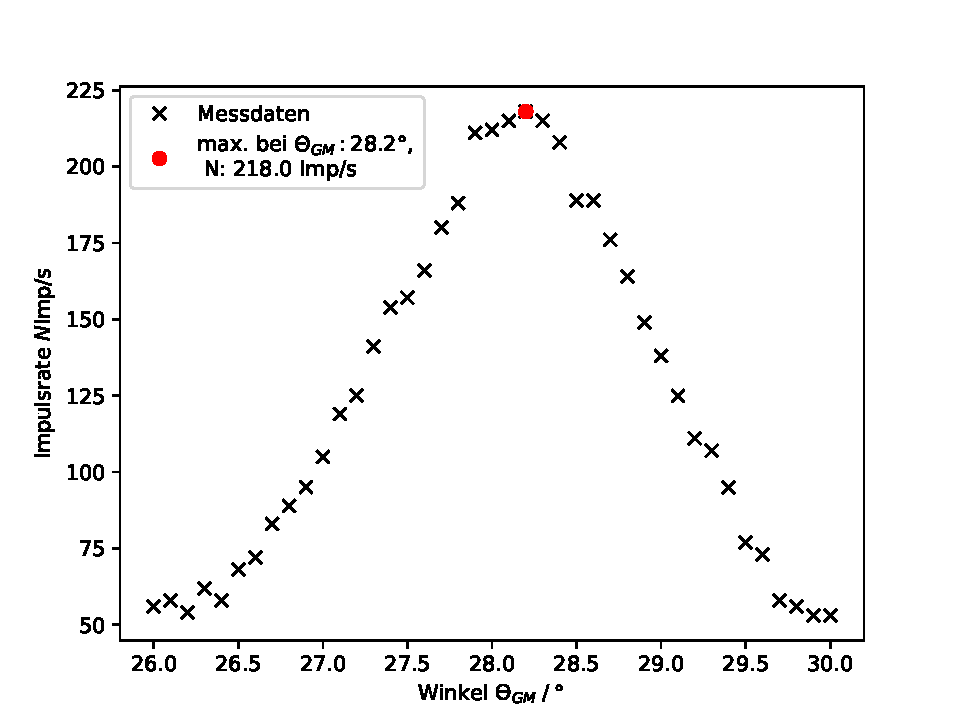
\includegraphics[width=0.7\textwidth]{plots/messdaten1.pdf}
    \caption{Die Intensitätsratenverteilung bei einem festen Kristallwinkel
    von $\Theta=14$° und mit varrierenden Geiger-Müller-Winkel $\Theta_{\text{GM}}$ mit makierten Maximum.}
    \label{fig:spektrums}
\end{figure}
\newpage
\subsection{Emissionspektrum}
Für das Emissionspektrum der Kupfer-Röntgenröhre ergibt sich mit Gl. \ref{eqn:bragg} die 
Wellenlänge $\lambda$ zu den Braggwinkeln $\Theta$.
\begin{figure}[H]
    \centering
    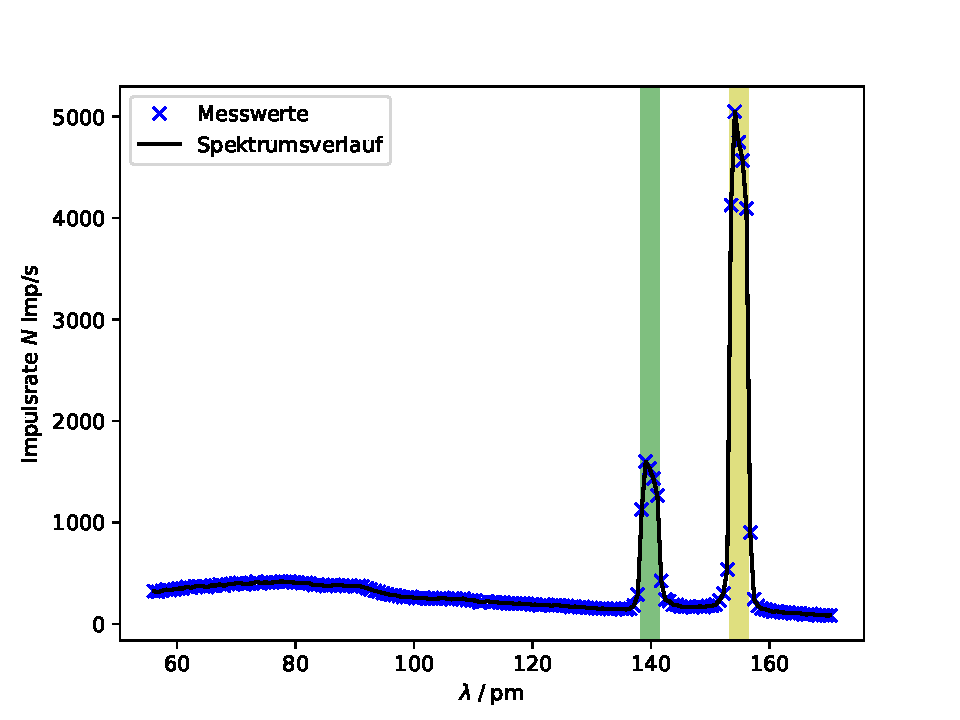
\includegraphics[width=0.7\textwidth]{plots/spektrum.pdf}
    \caption{Das Spektrum der Kupferanode. Dabei ist der erste Peak (in grün)
    die $K_{\beta}$ und der zweite Peak (in gelb) die $K_{\alpha}$ 
    Linie.}
    \label{fig:peaks}
\end{figure}
Mit den Halbwertsbreiten (vgl. Abs \ref{subsec:halbwert}) und den Energien $E_K$ und dessen Halbwertsenenergien $\Delta E_{\text{FWHM}}$
ergibt sich das Auflösungsvermögen $A$ über
\begin{equation}
    A=\frac{E_K}{\Delta E_{\text{FWHM}}}.
\end{equation}
\begin{table}[H]
    \centering
    \begin{tabular}{c | c c c c}
        \toprule
        & $E_K\;/\;\si{keV}$ & HB$\;/\;$pm & HE $\Delta E_{\text{FMWH}}\;/\;$eV&$A$\\
        \midrule
        $K_{\alpha}$ & 8,05 & 14,99 & 165,76 &48,56\\
        $K_{\beta}$  & 8,92 & 3,24  & 205,74 &43,36\\
        \bottomrule
    \end{tabular}
    \caption{Darstellung der Energien am Peak $E_K$ mit den zugehörigen Halbwertsbreiten
    HB, den Halbwertsenergien HE und dem Auflösungsvermögen $A$}
    \label{tab:tabelle1}
\end{table}
\subsection{Abschirmzahl}
Die Abschirmkonstanten $\sigma$ ergeben sich über Gl. \ref{eqn:sigma} mit $E_{\text{abs}}=8980\si{eV}$\cite{anleitung}
und $E_{\alpha}$ und $E_{\beta}$ aus Tabelle \ref{tab:tabelle1} zu
\begin{align*}
    \sigma_{K1}=&3,32,\\
    \sigma_{K2}=&12,47,\\
    \sigma_{K3}=&22,7.\\
\end{align*}
\subsection{Absorber}
Nun werden die Absorber mit dem Material Brom, Zink, Rubidium, Gallium, Rubidium und Strontium
zwischen den LiF-Kristall und den Geiger-Müller-Zähler gestellt.
Die Materiale haben folgende Kenngrößen.
\begin{table}
    \centering
    \begin{tabular}{c | c c c c}
        \toprule
        &$Z$ & $E_K^{Lit}\;/\;$keV & $\Theta_K^{Lit}\;/\;$° & $\sigma_K$\\
        \midrule
        Zn & 30 & 9,65 & 18,6 & 3,56\\
        Ga & 31 & 10,37 & 17,27 &3,62\\
        Br & 35 & 13,47 & 13,20 &3,85\\
        Rb & 37 & 15,20 & 11,70 &3,95\\
        Sr & 38 & 16,10 & 11,00 &4,01\\
        Zr & 40 & 17,99 & 9,6 & 4,11\\
        \bottomrule
    \end{tabular}
    \caption{Kenngrößen zu den verschiedenen Absorbermaterialien.\cite{Absorptionskanten}\\
    $Z$: Ordnungszahl\\
    $E_K^{Lit}$: Literaturwert der K-Kante\cite{Absorptionskanten}\\
    $\Theta_K^{Lit}$: Braggwinkel zu $E_K^{Lit}$\\
    $\sigma_K$: Abschirmkonstante}
    \label{tab:kenngroesse}
\end{table}

Zunächst wird die Impulsrate der einzelnen Absorbermaterialien gegen den zugehörigen
Bragg-Winkel augetragen (siehe Abs. \ref{subsec:anhang1}).\\ Aus diesen Absorbtionsspektren, welche die K-Kanten enthalten, können
die zugehörigen Energien $E_K$ bestimmt werden.\\
Die Mitte der K-Kante wird der Intensität $I_K$ zugeordnet, die sich
über die Mitte zwischen dem Intensitätsmaximum und Minimum definiert
\begin{equation}
    I_K=I_K^{min}+\frac{I_K^{max}-I_K^{min}}{2},
    \label{eqn:intensität}
\end{equation}
Über den zugehörigen Winkel $\Theta$ kann nun mithilfe der zugehörigen Wellenlänge
Gl. \ref{eqn:bragg} die Absorbtionsenergie $E_{K,abs}$ der K-Kante ermittelt werden.
Weiterführend folgt daraus nach Gl. \ref{eqn:sigmaZ} die K-Schlalen zugehörigen Abschirmkonstante $\sigma_K$.\\\\
Es ergibt sich für die verschiedenen Absorbermaterialien:
\begin{table}
    \centering
    \begin{tabular}{c | c c c c c c}
        \toprule
        &$\Theta\;/\;$° & $E_{\text{K,abs}}\,/\;$keV & $I_K^{\text{min}}\;/\;\frac{Imp}{s}$ & $I_K^{\text{max}}\;/\;\frac{Imp}{s}$ & $I_K\;/\;\frac{Imp}{s}$ & $\sigma_K$\\
        \midrule
        Brom & 13,2 & 13,49 & 9,0 & 27,0 & 18,0 & 3,84\\
        Zink & 18,7 & 9,61 & 55,0 & 102,0 & 78,5 & 3,64\\
        Gallium & 17,375 & 10,34 & 66,0 & 121,0 & 93,5 & 3,70\\
        Rubidium & 11,8 & 15,06 & 12,0 & 64,0 & 38,0 & 4,11\\
        Strontium & 11,1 & 16,00 & 50,0 & 193,0 & 121,5 & 4,12\\
        Zirkonium & 9,95 & 17,83 & 112,0 & 282,0 & 197,0 & 4,28\\
        \bottomrule
    \end{tabular}
    \caption{Die Lage der Absorbtionskante und Absorbtionsenergie $E_{K,abs}$ von Brom.
        Sowie die zugehörigen Intensitäten $I_K^{min}$,$I_K^{max}$,$I_K$ und die Abschirmkonstante $\sigma$.}
\end{table}
\newpage
Mithilfe Gl. \ref{eqn:mos} kann nun über eine Ausgleichsgerade
\begin{equation}
        \sqrt{E_K}=A\cdot Z +B,
\end{equation}
mit
\begin{align}
    A=\sqrt{R\cdot h},
    \label{eqn:Ry}
\end{align}
die Rydbergfrequenz $R$ nach Gl. \ref{eqn:Ry} bestimmt werden.
Für die Paramter der Ausgleichsgeraden ergibt sich
\begin{align*}
    B&=(-3,4\pm 0,4)\cdot 10^{-9}\sqrt{\si{eV}},\\
    A&=(1,432\pm 0,012) 10^{-9}\sqrt{\si{eV}}.\\
\end{align*}
\begin{figure}[H]
    \centering
    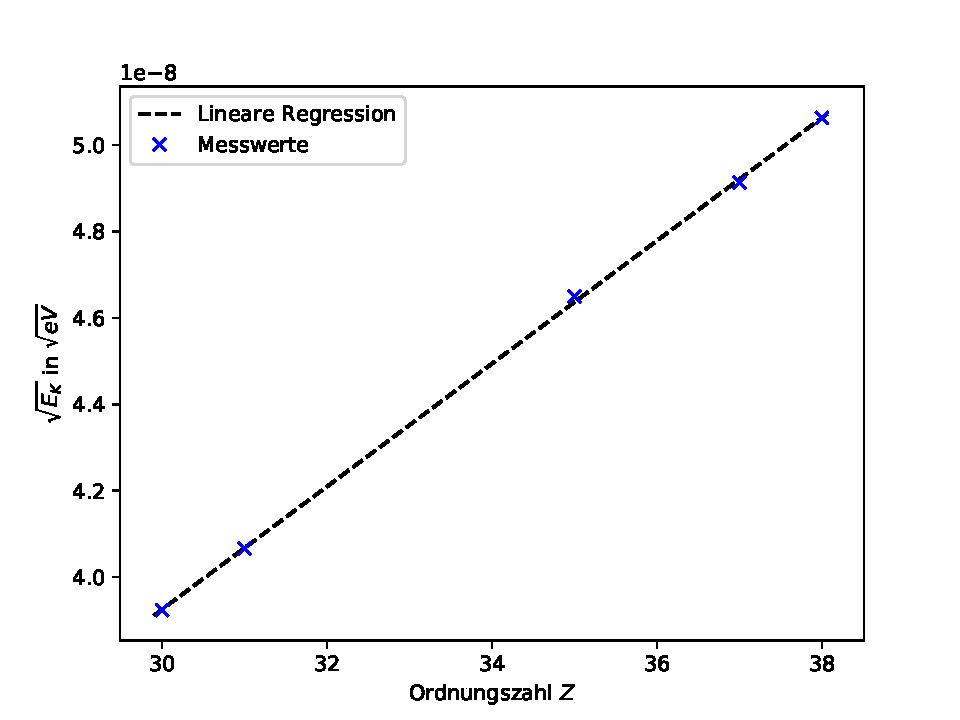
\includegraphics[width=0.7\textwidth]{plots/Moseley.pdf}
    \caption{$\sqrt{E_K}$ gegen die Ordnungzahl $Z$ der verschiedenen Absorbermaterialien
    aufgetragen. Aus der Steigung kann nun eine Aussage über die Rydberg-Konstant getroffen werden.}
\end{figure}
Es folgt somit für die Rydbergfrequenz, Rydbergkonstante, Rydbergenergie
\begin{align*}
    R_{\text{Frequenz}}&=\frac{A^2}{h}=(3,05\pm 0,05)\cdot 10^{15}\si{Hz},\\
    R_{\text{Energie}}&=R_{\infty}=\frac{R_{\text{Frequenz}}\cdot h}{e}=(12,63\pm 0,22)\si{eV},\\
    R_{\text{Konstant}}&=\frac{R_{\text{Frequenz}}}{c}=(1,018\pm 0,018)\cdot 10^7\frac{1}{m}.
\end{align*}

\label{sec:Auswertung}
